\documentclass[11pt,a4paper]{article}

\usepackage[T1]{fontenc}
\usepackage[margin=1in]{geometry}
\usepackage{amsmath}
\usepackage{amssymb}
\usepackage{array}
\usepackage{booktabs}
\usepackage{longtable}
\usepackage{xcolor}
\usepackage{tikz}
\usetikzlibrary{arrows.meta,positioning,calc,shapes.geometric}

\title{ELEC5803 HLS Exam Study\\Step-by-Step Solution to Question 2}
\author{}
\date{}

\tikzset{
  >={Latex[length=2mm]},
  block/.style={draw, rounded corners, align=center, minimum width=2.2cm, minimum height=0.9cm},
  reg/.style={draw, rounded corners, fill=blue!6, align=center, minimum width=1.2cm, minimum height=0.8cm},
  mul/.style={draw, circle, minimum size=8mm, inner sep=0pt, align=center, fill=green!6},
  add/.style={draw, circle, minimum size=8mm, inner sep=0pt, align=center, fill=orange!8},
  fu/.style={draw, rounded corners, fill=green!7, align=center, minimum width=2.5cm, minimum height=0.9cm},
  ctrl/.style={draw, rounded corners, fill=orange!10, align=center, minimum width=2.5cm, minimum height=0.9cm},
}

\begin{document}
\maketitle

\section*{Course-slide basis}
This solution follows the same course method used in:
\begin{itemize}
  \item \textbf{Slides 8}: FIR realization and multiplier sharing ideas in \texttt{Slides/ELEC5803\_Slides8\_Design Examples-Part1.pdf}.
  \item \textbf{Slides 9}: interval arithmetic, fixed-point representation, and computational-noise analysis in \texttt{Slides/ELEC5803\_Slides9\_Computing With Uncertainty.pdf}.
\end{itemize}

\section*{1. Interpreting the circuit}
The figure is a standard 4-tap direct-form FIR filter:
\[
y[n]=a_0x[n]+a_1x[n-1]+a_2x[n-2]+a_3x[n-3].
\]
The three delay blocks $R_1$, $R_2$, and $R_3$ store the previous input samples; the four multipliers $M_0$--$M_3$ scale the current and delayed samples; and the three adders $A_1$--$A_3$ accumulate the four products.

\begin{figure}[h!]
\centering
\resizebox{\textwidth}{!}{%
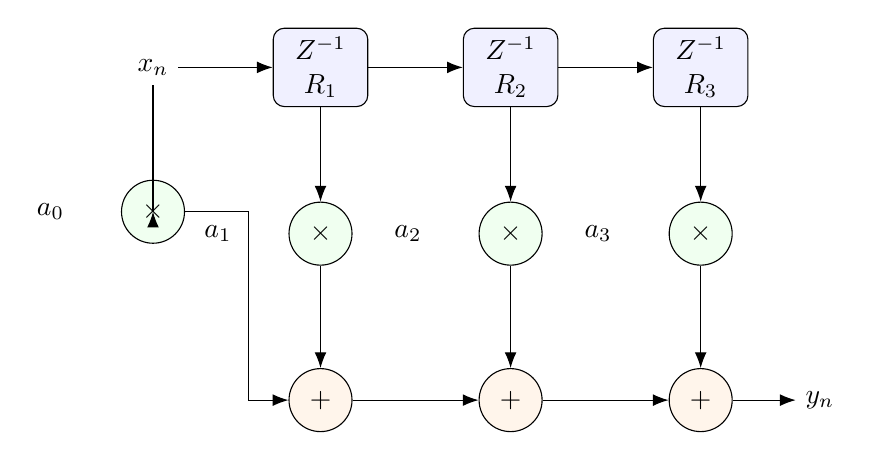
\begin{tikzpicture}[node distance=9mm and 10mm]
  \node (xin) {$x_n$};
  \node[reg, right=12mm of xin] (r1) {$Z^{-1}$\\$R_1$};
  \node[reg, right=12mm of r1] (r2) {$Z^{-1}$\\$R_2$};
  \node[reg, right=12mm of r2] (r3) {$Z^{-1}$\\$R_3$};

  \node[mul, below=12mm of xin] (m0) {$\times$};
  \node[mul, below=12mm of r1] (m1) {$\times$};
  \node[mul, below=12mm of r2] (m2) {$\times$};
  \node[mul, below=12mm of r3] (m3) {$\times$};

  \node[add, below=13mm of m1] (a1) {$+$};
  \node[add, below=13mm of m2] (a2) {$+$};
  \node[add, below=13mm of m3] (a3) {$+$};
  \node[right=8mm of a3] (yout) {$y_n$};

  \node[left=6mm of m0] {$a_0$};
  \node[left=6mm of m1] {$a_1$};
  \node[left=6mm of m2] {$a_2$};
  \node[left=6mm of m3] {$a_3$};

  \draw[->] (xin) -- (r1);
  \draw[->] (r1) -- (r2);
  \draw[->] (r2) -- (r3);

  \draw[->] (xin) |- (m0);
  \draw[->] (r1) -- ++(0,-6mm) -| (m1);
  \draw[->] (r2) -- ++(0,-6mm) -| (m2);
  \draw[->] (r3) -- ++(0,-6mm) -| (m3);

  \draw[->] (m0.east) -- ++(8mm,0) |- (a1.west);
  \draw[->] (m1) -- (a1);
  \draw[->] (a1.east) -- ++(8mm,0) |- (a2.west);
  \draw[->] (m2) -- (a2);
  \draw[->] (a2.east) -- ++(8mm,0) |- (a3.west);
  \draw[->] (m3) -- (a3);
  \draw[->] (a3) -- (yout);
\end{tikzpicture}%
}
\caption{Native-LaTeX redrawing of the 4-tap FIR filter in Q2.}
\end{figure}

\section*{2. Part (a): interval analysis and required bit-widths}
\subsection*{2.1 Given input intervals}
\[
\begin{aligned}
a_0 &\in [-50.01,100.01], \\
a_1 &\in [-200.01,60.5], \\
a_2 &\in [-50.01,130.1], \\
a_3 &\in [-25.01,240.01], \\
x[n] &\in [-100.01,100.01].
\end{aligned}
\]

Because the delay elements only store previous input samples,
\[
x[n-1],\,x[n-2],\,x[n-3]\in[-100.01,100.01].
\]
So every memory unit $R_i$ must at least represent the same range as the input.

\subsection*{2.2 Interval rule used}
From Slides 9, interval arithmetic represents each quantity by a lower and upper bound. For multiplication:
\[
[a,b]\cdot[c,d]=[\min(ac,ad,bc,bd),\max(ac,ad,bc,bd)].
\]
For addition:
\[
[a,b]+[c,d]=[a+c,b+d].
\]

\subsection*{2.3 Multiplier ranges}
\paragraph{Multiplier $M_0$:}
\[
a_0x[n]=[-50.01,100.01]\cdot[-100.01,100.01].
\]
Endpoint products:
\[
\begin{aligned}
(-50.01)(-100.01)&=5001.5001,\\
(-50.01)(100.01)&=-5001.5001,\\
(100.01)(-100.01)&=-10002.0001,\\
(100.01)(100.01)&=10002.0001.
\end{aligned}
\]
Therefore,
\[
M_0\in[-10002.0001,10002.0001].
\]

\paragraph{Multiplier $M_1$:}
\[
a_1x[n-1]=[-200.01,60.5]\cdot[-100.01,100.01].
\]
Endpoint products:
\[
\begin{aligned}
(-200.01)(-100.01)&=20003.0001,\\
(-200.01)(100.01)&=-20003.0001,\\
(60.5)(-100.01)&=-6050.605,\\
(60.5)(100.01)&=6050.605.
\end{aligned}
\]
Hence,
\[
M_1\in[-20003.0001,20003.0001].
\]

\paragraph{Multiplier $M_2$:}
\[
a_2x[n-2]=[-50.01,130.1]\cdot[-100.01,100.01].
\]
Endpoint products give
\[
M_2\in[-13011.3010,13011.3010].
\]

\paragraph{Multiplier $M_3$:}
\[
a_3x[n-3]=[-25.01,240.01]\cdot[-100.01,100.01].
\]
Endpoint products give
\[
M_3\in[-24003.4001,24003.4001].
\]

\subsection*{2.4 Adder ranges}
The adders accumulate the multiplier outputs from left to right.

\paragraph{Adder $A_1$:}
\[
A_1=M_0+M_1.
\]
So,
\[
A_1\in[-10002.0001,10002.0001]+[-20003.0001,20003.0001]
=[-30005.0002,30005.0002].
\]

\paragraph{Adder $A_2$:}
\[
A_2=A_1+M_2.
\]
Thus,
\[
A_2\in[-30005.0002,30005.0002]+[-13011.3010,13011.3010]
=[-43016.3012,43016.3012].
\]

\paragraph{Adder $A_3$:}
\[
A_3=A_2+M_3.
\]
Hence,
\[
A_3\in[-43016.3012,43016.3012]+[-24003.4001,24003.4001]
=[-67019.7013,67019.7013].
\]

\subsection*{2.5 Required signed bit-widths}
Following the bit-width method used in the slides, we choose the smallest signed word length whose range contains the maximum absolute value.

\begin{center}
\begin{tabular}{lcc}
\toprule
Unit & Interval range & Minimum signed bit-width \\
\midrule
$R_1,R_2,R_3$ & $[-100.01,100.01]$ & 8 bits \\
$M_0$ & $[-10002.0001,10002.0001]$ & 15 bits \\
$M_1$ & $[-20003.0001,20003.0001]$ & 16 bits \\
$M_2$ & $[-13011.3010,13011.3010]$ & 15 bits \\
$M_3$ & $[-24003.4001,24003.4001]$ & 16 bits \\
$A_1$ & $[-30005.0002,30005.0002]$ & 16 bits \\
$A_2$ & $[-43016.3012,43016.3012]$ & 17 bits \\
$A_3$ & $[-67019.7013,67019.7013]$ & 18 bits \\
\bottomrule
\end{tabular}
\end{center}

\subsection*{2.6 Final answer for part (a)}
\[
\boxed{
\begin{aligned}
R_i &: 8\text{ bits},\\
M_0 &: 15\text{ bits},\quad M_1:16\text{ bits},\quad M_2:15\text{ bits},\quad M_3:16\text{ bits},\\
A_1 &: 16\text{ bits},\quad A_2:17\text{ bits},\quad A_3:18\text{ bits}.
\end{aligned}}
\]

\section*{3. Part (b): computational noise for 16-bit fixed-point (10.6)}
\subsection*{3.1 Assumption used}
The course slides use a simplified additive-noise model:
\begin{itemize}
  \item each arithmetic unit is ideal followed by a quantization error source,
  \item if rounding is used, each arithmetic operation contributes at most $\pm 0.5$ LSB.
\end{itemize}

For a \texttt{(10.6)} format:
\[
\text{LSB}=2^{-6}=\frac{1}{64}=0.015625.
\]
Therefore, the maximum rounding noise per operation is
\[
\pm 0.5\,\text{LSB}=\pm 2^{-7}=\pm 0.0078125.
\]

\subsection*{3.2 Count the arithmetic operations}
Per output sample, this FIR structure performs:
\begin{itemize}
  \item 4 multiplications,
  \item 3 additions.
\end{itemize}
So the total number of finite-precision arithmetic operations is
\[
4+3=7.
\]

\subsection*{3.3 Worst-case output noise}
Using the same worst-case accumulation style as the slide examples:
\[
e_{\max}=7\times 0.5\,\text{LSB}=7\times 0.0078125=0.0546875.
\]
Equivalently,
\[
e_{\max}=\pm 3.5\ \text{LSB}.
\]

\subsection*{3.4 Final answer for part (b)}
\[
\boxed{\text{Maximum output computational noise} \approx \pm 0.0546875\;(\pm 3.5\ \text{LSB})}
\]

\noindent
This is the \emph{slide-style worst-case arithmetic-noise estimate}. A more detailed model could also include separate coefficient/data quantization terms, but the exam statement does not provide a single concrete coefficient set for part (b), so the direct slide-based answer is the operation-noise bound above.

\section*{4. Part (c): minimum-component implementation with no computational error}
\subsection*{4.1 Given constant coefficients}
Now the FIR is
\[
y[n]=24x[n]+65x[n-1]+63x[n-2]+48x[n-3].
\]

The key idea from the FIR design examples in Slides 8 is:
\begin{itemize}
  \item replace constant multipliers by shifts and adds/subtracts whenever possible,
  \item then share arithmetic hardware to minimize the number of components.
\end{itemize}

\subsection*{4.2 Rewrite the equation to expose sharing}
Start with
\[
y[n]=24x_0+65x_1+63x_2+48x_3
\]
where
\[
x_0=x[n],\quad x_1=x[n-1],\quad x_2=x[n-2],\quad x_3=x[n-3].
\]

Observe:
\[
65x_1+63x_2=64x_1+x_1+64x_2-x_2=64(x_1+x_2)+(x_1-x_2).
\]
Also,
\[
24x_0+48x_3=24(x_0+2x_3).
\]
Therefore,
\[
\boxed{y[n]=64(x_1+x_2)+(x_1-x_2)+24(x_0+2x_3)}.
\]

Now rewrite the constant multiplications as shifts:
\[
64u=u\ll 6,\qquad 24v=(v\ll 4)+(v\ll 3).
\]
So the final computation becomes
\[
\boxed{
y[n]=\big((x_1+x_2)\ll 6\big)+(x_1-x_2)+\big((x_0+2x_3)\ll 4\big)+\big((x_0+2x_3)\ll 3\big).
}
\]

\subsection*{4.3 Why this removes computational error}
This implementation is exact because:
\begin{itemize}
  \item all coefficients are integers,
  \item multiplication by powers of two is just a left shift,
  \item the remaining operations are only additions and one subtraction,
  \item no coefficient approximation is needed.
\end{itemize}
So there is \textbf{no coefficient quantization error}. To avoid overflow, we only need sufficient internal/output bit-width.

\subsection*{4.4 Output range for part (c)}
Since all coefficients are positive and the input range is symmetric:
\[
|y[n]|_{\max}=(24+65+63+48)\times 100.01 = 200\times 100.01 = 20002.
\]
Hence,
\[
y[n]\in[-20002,20002].
\]
So the final output requires at least
\[
\boxed{16\text{ signed bits}}
\]
for the integer-range part, because a signed 16-bit value covers $[-32768,32767]$.

\subsection*{4.5 Minimum-component datapath}
To minimize hardware components, use:
\begin{itemize}
  \item three delay registers for the FIR memory,
  \item one shifter unit,
  \item one shared adder/subtractor/accumulator,
  \item a few temporary registers,
  \item one FSM controller.
\end{itemize}

\begin{figure}[h!]
\centering
\resizebox{\textwidth}{!}{%
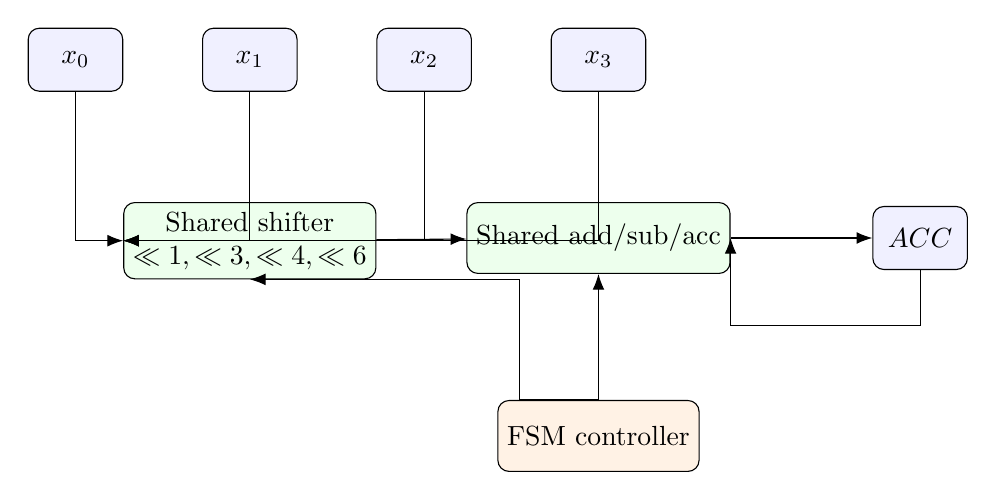
\begin{tikzpicture}[node distance=9mm and 10mm]
  \node[reg] (x0) {$x_0$};
  \node[reg, right=10mm of x0] (x1) {$x_1$};
  \node[reg, right=10mm of x1] (x2) {$x_2$};
  \node[reg, right=10mm of x2] (x3) {$x_3$};

  \node[fu, below=14mm of x1] (shift) {Shared shifter\\$\ll 1,\ll 3,\ll 4,\ll 6$};
  \node[fu, below=14mm of x3] (alu) {Shared add/sub/acc};
  \node[reg, right=18mm of alu] (acc) {$ACC$};
  \node[ctrl, below=16mm of alu] (fsm) {FSM controller};

  \draw[->] (x0.south) -- ++(0,-6mm) |- (shift.west);
  \draw[->] (x1.south) -- ++(0,-6mm) |- (shift.west);
  \draw[->] (x2.south) -- ++(0,-6mm) |- (shift.west);
  \draw[->] (x3.south) -- ++(0,-6mm) |- (shift.west);
  \draw[->] (shift) -- (alu);
  \draw[->] (alu) -- (acc);
  \draw[->] (acc.south) -- ++(0,-7mm) -| (alu.east);
  \draw[->] (fsm.north) -- (alu.south);
  \draw[->] (fsm.north) -- ++(-10mm,0) |- (shift.south);
\end{tikzpicture}%
}
\caption{Area-minimized hardware for part (c): a shift-add/sub FSMD.}
\end{figure}

\subsection*{4.6 One exact micro-operation schedule}
Using the algebra above, one output sample can be computed as:
\begin{center}
\begin{tabular}{cl}
\toprule
Step & Operation \\
\midrule
1 & $t_1 \leftarrow x_1 + x_2$ \\
2 & $t_2 \leftarrow x_1 - x_2$ \\
3 & $p_{12} \leftarrow (t_1 \ll 6) + t_2$ \\
4 & $t_3 \leftarrow x_0 + (x_3 \ll 1)$ \\
5 & $p_{03} \leftarrow (t_3 \ll 4) + (t_3 \ll 3)$ \\
6 & $y \leftarrow p_{12} + p_{03}$ \\
\bottomrule
\end{tabular}
\end{center}

This realizes the filter exactly with no general multipliers.

\subsection*{4.7 Final answer for part (c)}
An efficient minimum-component exact implementation is:
\begin{itemize}
  \item use the transformed equation
  \[
  y[n]=64(x_1+x_2)+(x_1-x_2)+24(x_0+2x_3),
  \]
  \item realize multiplications only by left shifts,
  \item use one shared adder/subtractor/accumulator plus one shared shifter under FSM control,
  \item size the final output path for at least 16 signed bits.
\end{itemize}

\section*{5. Final exam-style summary}
\subsection*{(a)}
Using interval arithmetic:
\[
\boxed{
R_i:8,\;
M_0:15,\;
M_1:16,\;
M_2:15,\;
M_3:16,\;
A_1:16,\;
A_2:17,\;
A_3:18\ \text{bits}
}
\]

\subsection*{(b)}
For 16-bit fixed-point \texttt{(10.6)} arithmetic:
\[
\boxed{e_{\max}\approx \pm 3.5\ \text{LSB}=\pm 0.0546875.}
\]

\subsection*{(c)}
Use coefficient decomposition and hardware sharing:
\[
\boxed{y[n]=64(x_1+x_2)+(x_1-x_2)+24(x_0+2x_3)}
\]
which leads to an exact shift-add implementation with no general multipliers and no computational error.

\end{document}
